
\begin{figure}[H]
    \vspace{8mm}
    \begin{minipage}{0.5\textwidth}
        \begin{circuitikz}[scale=1, transform shape] 
            \draw
              % MOSFET transistor with labels for drain (D), gate (G), source (S), and bulk (B)
              (0,0) node[nmos, bulk] (mos) {}
              (mos.drain) node[left] {M1}
            
              % Gate voltage source VGS
              (mos.gate) to[short, -] ++(-2,0) to[voltage source, l^=$V_{GS}$] ++(0,-1.5) node[ground] {}
              
              % Drain voltage source VDS (vertical)
              (mos.drain) to[short, -] ++(0,1) -- ++(2,0) -- ++(0,-1) to[voltage source, l^=$V_{DS} $] ++(0,-2) -- (2,-1.5) node[ground] {}
              
              % Source connected to ground, aligned with VGS ground
              (mos.source) to[short, -] (0,-1.5) node[ground] {}
              
              % Bulk (body) connection to ground
              (mos.bulk) to[short, -] (0.5, 0) -- ++(0,-1) -- ++(-0.5,0)  node[circle,fill,inner sep=1pt] (myNode) {}
            ;
        \end{circuitikz}

        \vspace{5mm}
        \centering{(NMOS)}
    \end{minipage}
    \hfill
    \begin{minipage}{0.5\textwidth}
        \begin{circuitikz}[scale=1, transform shape] 
            \draw
              % MOSFET transistor with labels for drain (D), gate (G), source (S), and bulk (B)
              (0,0) node[pmos, bulk] (mos) {}
              (mos.drain) node[left] {M1}
                          
              % Gate voltage source VGS
              (mos.gate) to[short, -] (-2,0) to[voltage source, l^=$V_{GS}$] (-2,2) -- ++(2,0) node[circle,fill,inner sep=1pt] (myNode) {}
              
              % Drain voltage source VDS (vertical)
              (mos.source) to[short, -] (0,2) -- ++(2,0) -- ++(0,-1) to[voltage source, l^=$V_{DS} $] ++(0,-2) -- (2,-1.5) -- (0,-1.5)
              
              % Source connected to ground, aligned with VGS ground
              (mos.drain) to[short, ] (0,-1.5) node[circle,fill,inner sep=1pt] (myNode) {} (0,-1.5) node[ground] {}

              % Bulk (body) connection to ground
              (mos.bulk) to[short, -] (0.5, 0) -- ++(0,1) -- ++(-0.5,0)  node[circle,fill,inner sep=1pt] (myNode) {}

            %   (2,2)  to[short, *-o] ++(1,0) node[above, right]{$V_{CC}$}
            ;
        \end{circuitikz}

        \vspace{5mm} 
        \centering{(PMOS)}
    \end{minipage}
    \caption{\label{cod:cod_NP_WL_const} Zapojení pro určení \(U_{TH0}\) pro tranzistor NMOS a PMOS}
\end{figure}

\begin{figure}[h]
    \hspace{-20mm}
    \begin{minipage}{0.5\textwidth}
        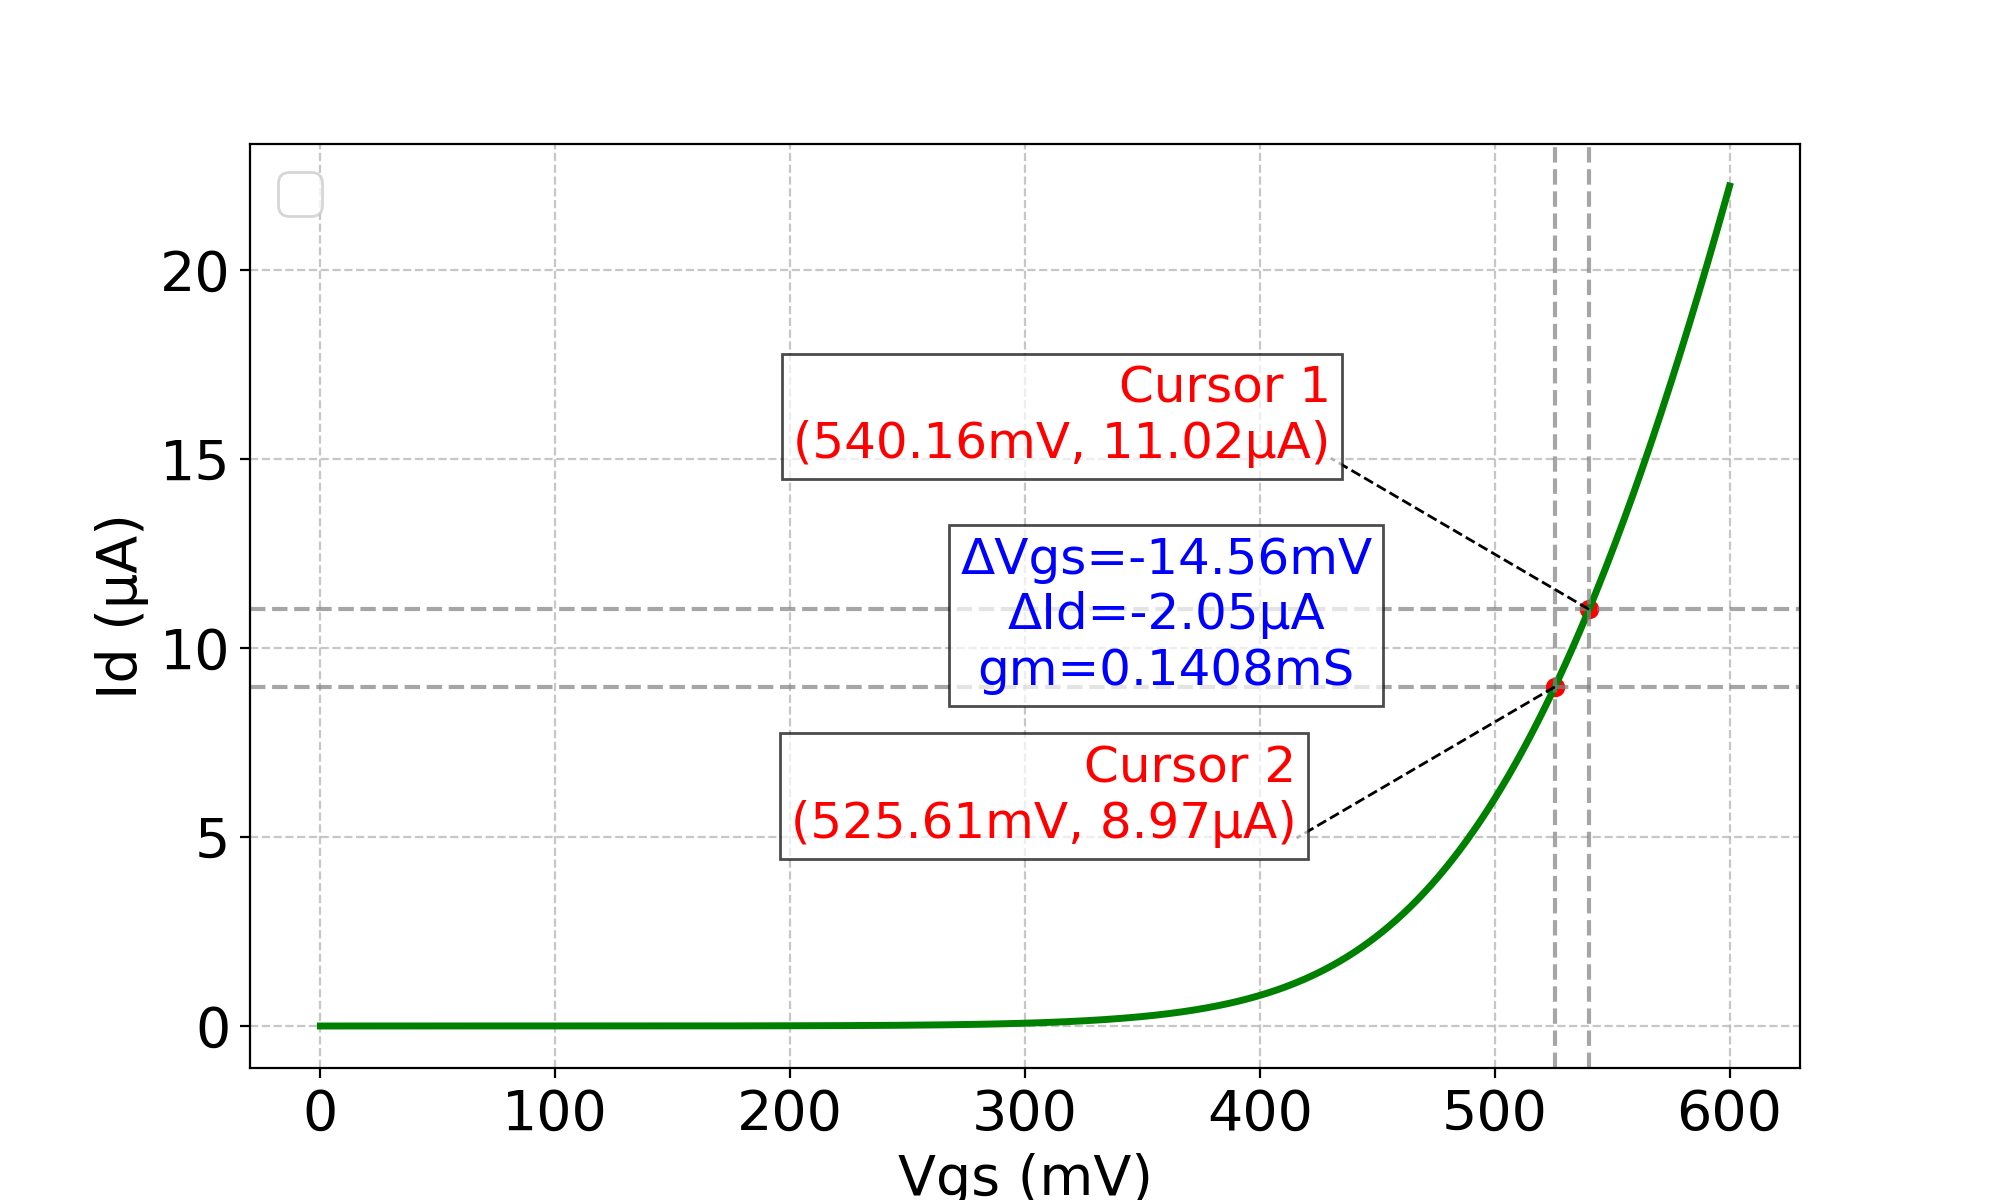
\includegraphics[height=0.25\textheight]{text/img/N-KP.png}
        \centering{(NMOS)}
    \end{minipage}
    \hfill
    \begin{minipage}{0.5\textwidth}
        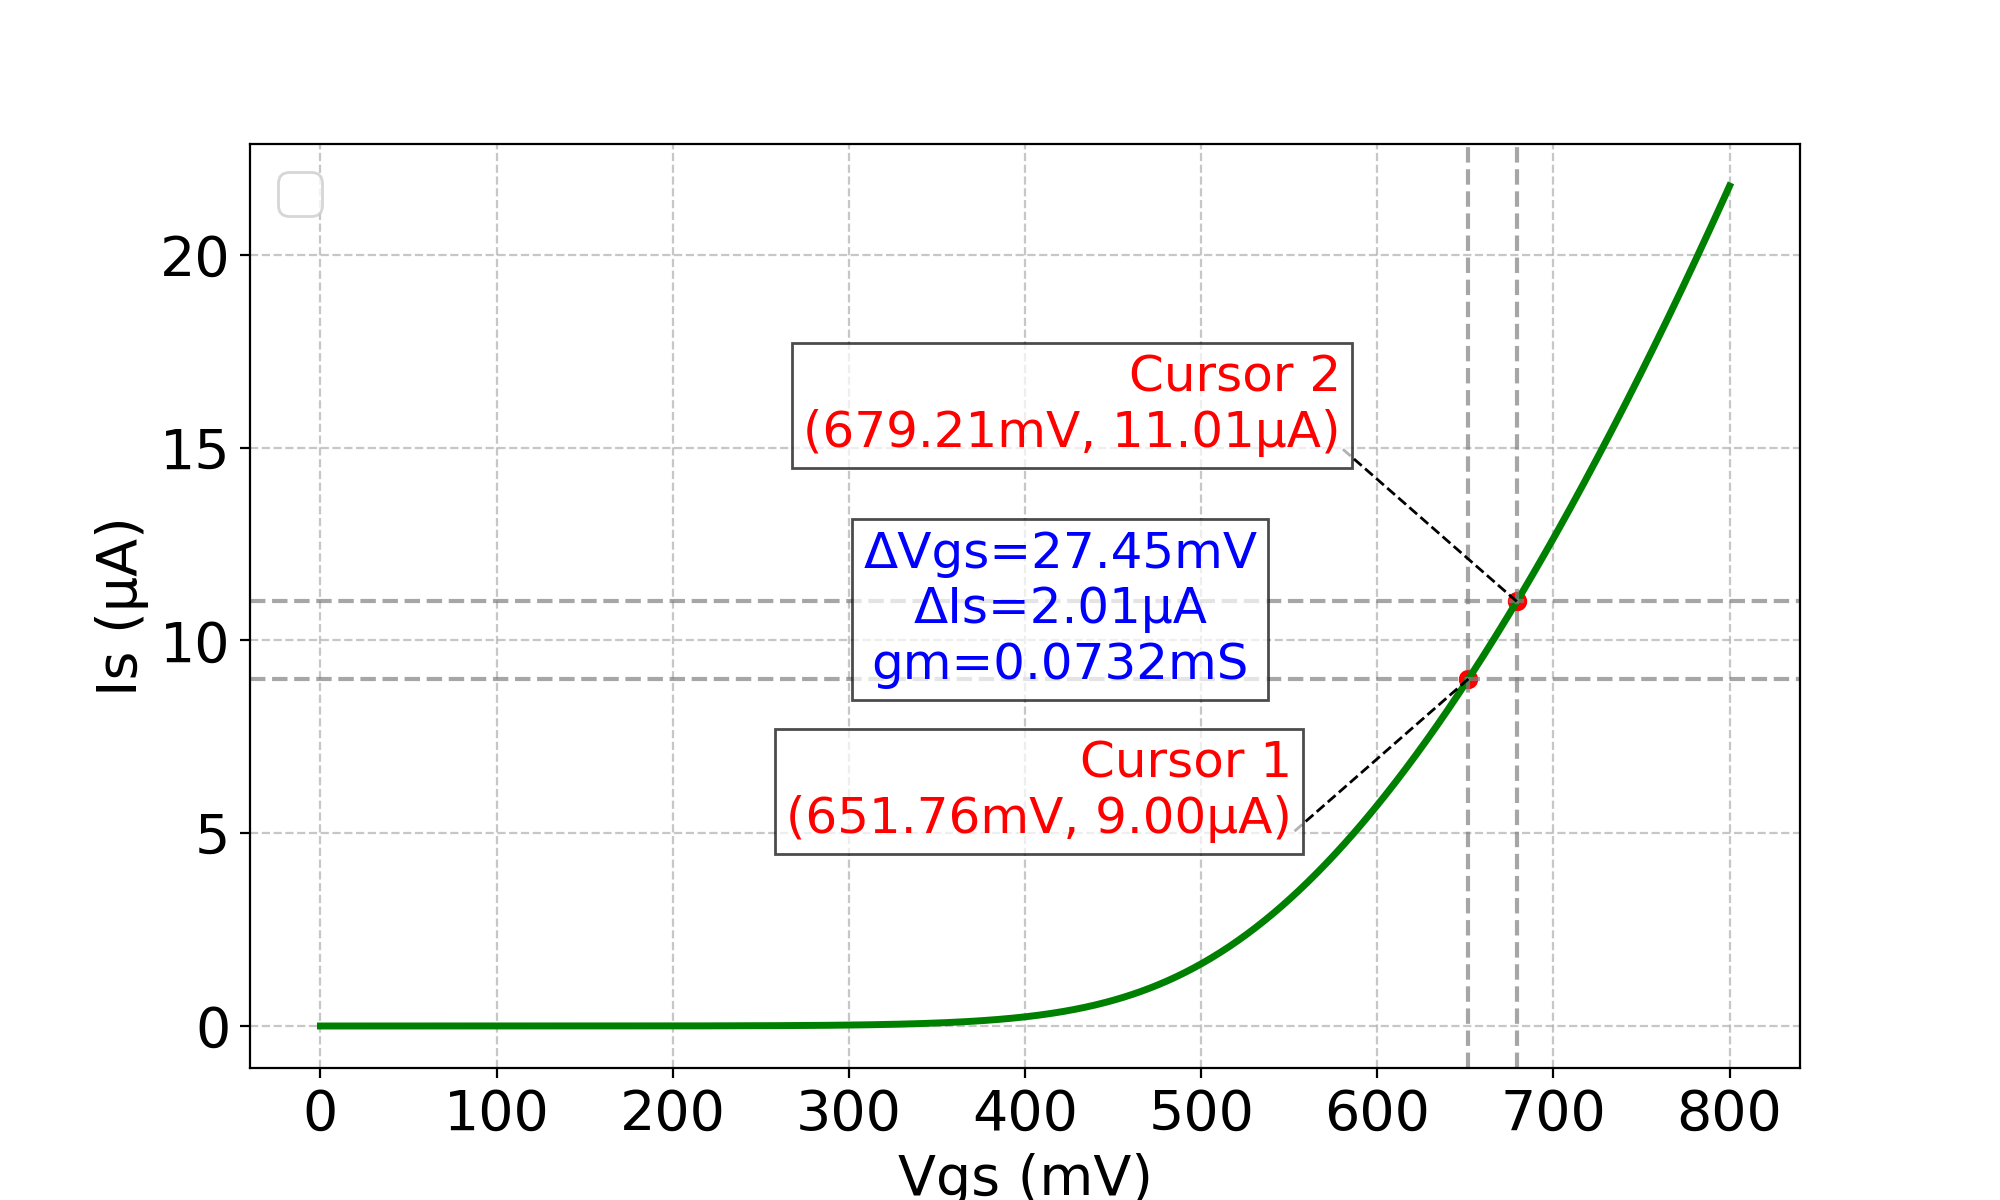
\includegraphics[height=0.25\textheight]{text/img/P-KP.png}
        \centering{(PMOS)}
    \end{minipage}
    \caption{\label{fig:graf_NP_KP} Závislost proudu tranzistorem NMOS i PMOS na napětí \(V_{GS}\)}
\end{figure}

Z uvedených kurzoru přímo vidímě strmost \(g_m\), \(140.8 \mu S\) pro NMOS a \(73.2 \mu S\) pro PMOS.
Mužeme tedy spočítat transkonduktanční parametr \(KP\) jako:\\


\Large
\(
    KP = \frac{g_m^2\cdot L}{2\cdot|I_D|\cdot W}
\)
\normalsize

Tedy pro NMOS:

\Large
\(
    KP_N = \frac{g_{m-N}^2\cdot L}{2\cdot|I_{D-N}|\cdot W} = \frac{(140.8\mu)^2\cdot1\mu}{2\cdot10\mu\cdot5\mu} = 198.2\mu A V^{-2} \cong 200 \mu A V^{-2}
\)
\normalsize

A PMOS:

\Large
\(
    KP_P = \frac{g_{m-P}^2\cdot L}{2\cdot|I_{D-P}|\cdot W} = \frac{(73.2\mu)^2\cdot1\mu}{2\cdot10\mu\cdot5\mu} = 53.6\mu A V^{-2} \cong  50 \mu A V^{-2}
\)
\normalsize